In this section we will use visualization method in order to explore the data variables
distribution and relationships.

\subsection{Variables}

After pre processing the data, the data set contains the following variables

\begin{table}[ht!]
\begin{center}
\begin{tabular}{llllrr}
\toprule
Variable &  Description & Type &\\
\midrule
     Previous Dialog Act & the dialog act before the current one  & categorical\\
     Dialog Act & the current dialog act & categorical \\
     Length & length of the current dialog act in seconds & seconds \\
     Relative Turn Length (RTL)  & Relative turn length as defined in \ref{sfeatures} & percent \\
     Relative Time Control (RTC) & Relative time control as defined in \ref{sfeatures} & percent \\
     Turn Change & 1 if there was a turn change after this dialog act & binary \\
\bottomrule
\end{tabular}
\end{center}
\caption{Data Fields}
\end{table}


\subsection{Dialog Acts}

Figure \ref{f1} shows the relative presence of each dialog act. We can observe that the majority of dialog acts are statements, backchannels and opinions. This is true to the nature of the switchboard corpus
which consists mainly of casual conversations.

 \begin{figure}[ht!]
 \centering
 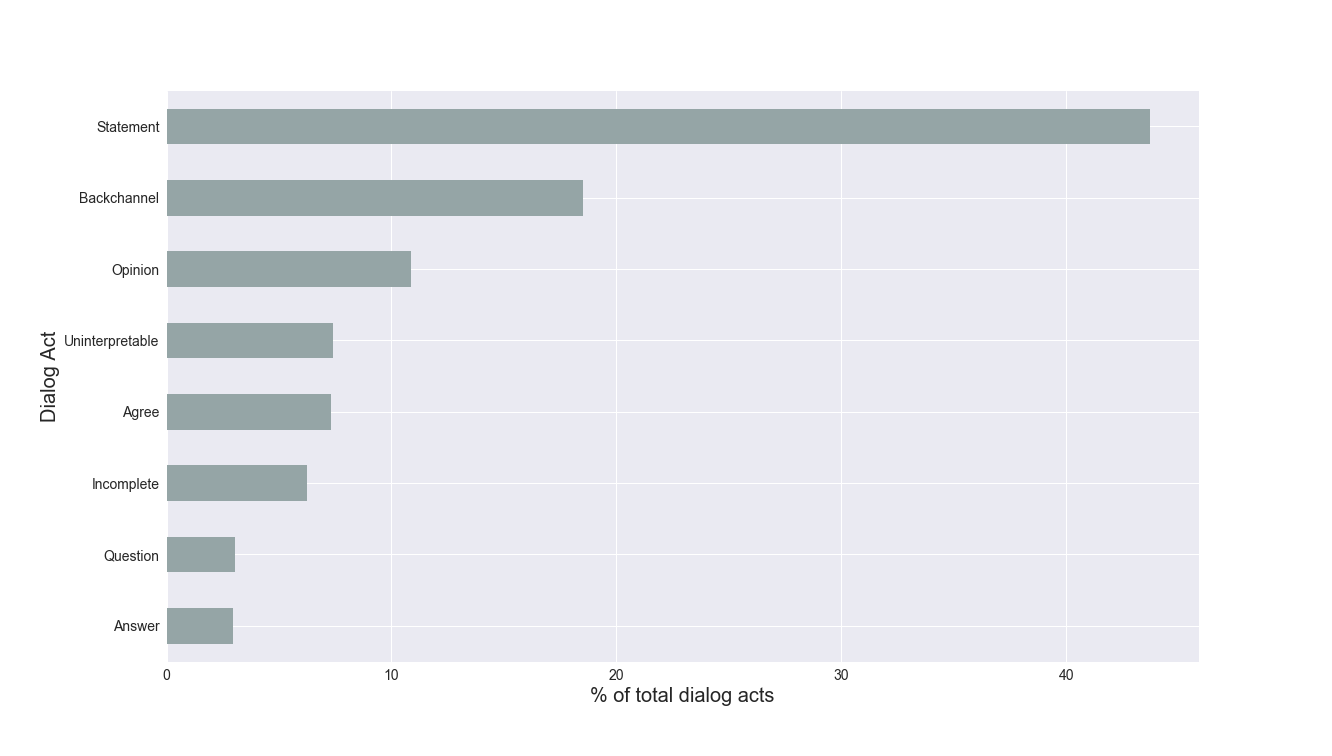
\includegraphics[width=\textwidth]{../scikitlearn/figures/f1.png}
 \caption{Dialog act relative count\label{overflow}}
 \label{f1}
 \end{figure}

In figure \ref{f2} , we measure the probability that a dialog act will lead to turn change. We can observe that the majority of back channels and question will lead to a turn change.

\begin{figure}[ht!]
\centering
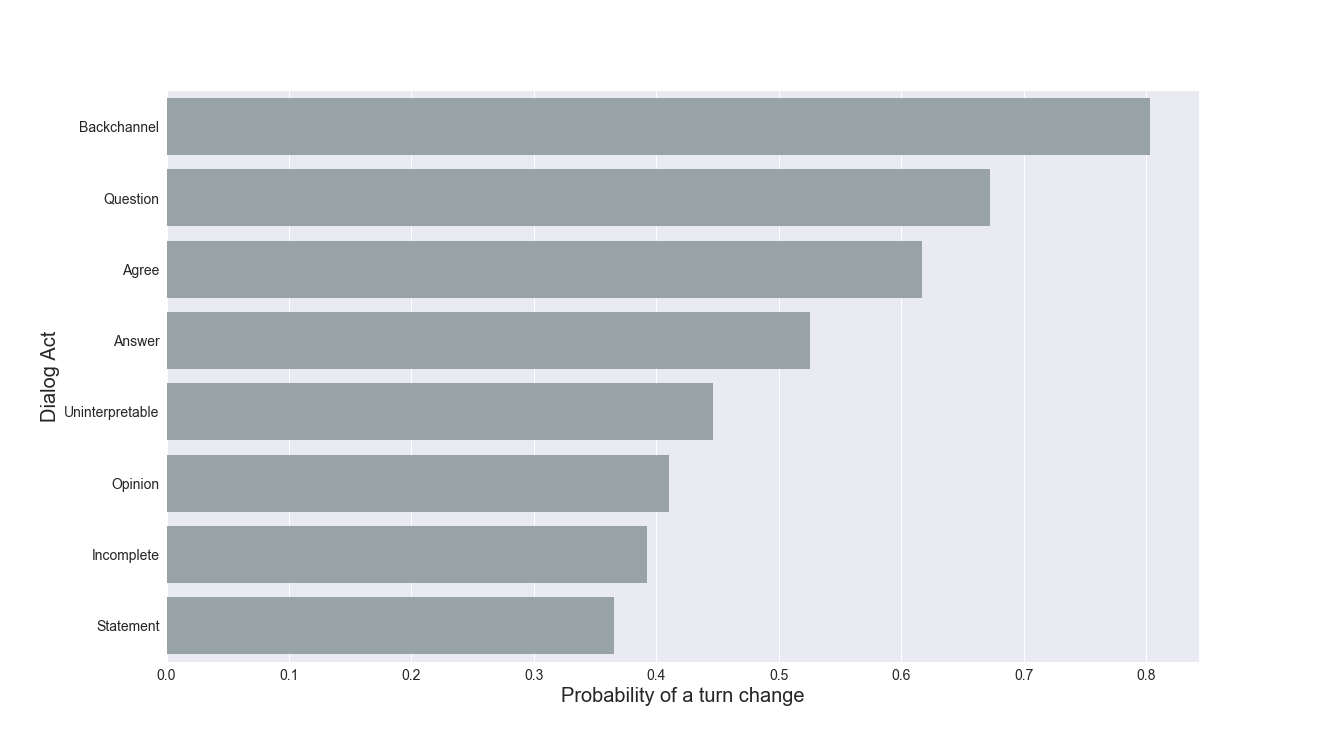
\includegraphics[width=\textwidth]{../scikitlearn/figures/f2.png}
\caption{Dialog act probability of turn change\label{overflow}}
\label{f2}
\end{figure}
\pagebreak 